\documentclass[12pt]{article}


\usepackage{amssymb}
\usepackage{amsmath}
\usepackage{fullpage}
\usepackage{epsfig}
\usepackage{epstopdf}
\everymath{\displaystyle}
\usepackage{enumerate}

\newif\ifans

\ansfalse

\begin{document}

\begin{center}
\underline{\LARGE{Triple Integrals}}
\end{center}

\noindent SUGGESTED REFERENCE MATERIAL:

\bigskip

\noindent As you work through the problems listed below, you should reference Chapters 14.5 \& 14.6 of the recommended textbook (or the equivalent chapter in your alternative textbook/online resource) and your lecture notes.

\bigskip

\noindent EXPECTED SKILLS:

\begin{itemize}

\item Be able to set up and evaluate triple integrals over rectangular boxes.

\item Know how to set up and evaluate triple integrals over more general regions by using Theorem 14.5.2 (projecting the solid onto the $xy$-plane), as well as by projecting the solid onto the $xz$- or $yz$-planes.

\item Be able to set up and evaluate triple integrals in spherical and cylindrical coordinates. Also, be able to convert integrals from rectangular coordinates to these other coordinate systems, remembering that $dV = r\,dzdrd\theta=\rho^2\sin\phi \,d\rho d\theta d\phi$.

\end{itemize}

\noindent PRACTICE PROBLEMS:

\medskip

\begin{enumerate}

\item Evaluate the following triple integrals.

\begin{enumerate}

\item $\int_1^3 \int_0^1 \int_0^z ye^{-z^3} \,dy\,dz\,dx$

\ifans{\fbox{$\frac{1}{3}\left(1-\frac{1}{e}\right)$}} \fi

\item $\iiint \limits_{G} z\sqrt{y} \,dV$, where $G$ is the solid exclosed by $z=y$, $y=x^2$, $y=4$, and the $xy$-plane.

\ifans{\fbox{64}} \fi

\end{enumerate}

\item Consider the region $G$ in 3-space which is enclosed by $z=0$, $z=1$, $x=0$, $y=x$, and $y=1-x$.  For each of the following, set up $\iiint \limits_{G} f(x,y,z)\,dV$ with the indicated order of integration.  Sketching $G$ may be helpful.

\begin{enumerate}

\item $dzdydx$

\ifans{\fbox{$\int_0^{1/2} \int_x^{1-x} \int_0^1 f(x,y,z) \,dz\,dy\,dx$}} \fi

\item $dzdxdy$

\ifans{\fbox{$\int_0^{1/2} \int_0^y \int_0^1 f(x,y,z) \,dz\,dx\,dy+\int_{1/2}^1 \int_0^{1-y} \int_0^1 f(x,y,z)\,dz\,dx\,dy$}} \fi

\item $dydzdx$

\ifans{\fbox{$\int_0^{1/2} \int_0^1 \int_x^{1-x} f(x,y,z) \,dy\,dz\,dx$}} \fi

\item $dydxdz$

\ifans{\fbox{$\int_0^1 \int_0^{1/2} \int_x^{1-x} f(x,y,z) \,dy\,dx\,dz$}} \fi

\item $dxdzdy$

\ifans{\fbox{$\int_0^{1/2} \int_0^1 \int_0^y f(x,y,z) \,dx\,dz\,dy+\int_{1/2}^1 \int_0^1 \int_0^{1-y} f(x,y,z)\,dx\,dz\,dy$}} \fi

\item $dxdydz$

\ifans{\fbox{$\int_0^1 \int_0^{1/2} \int_0^y f(x,y,z) \,dx\,dy\,dz+\int_0^1 \int_{1/2}^1 \int_0^{1-y} f(x,y,z)\,dx\,dy\,dz$}} \fi

\end{enumerate}

\item Consider the integral $I=\int_0^7 \int_0^{3-\frac{3}{7}x} \int_0^{21-3x-7y} 1 \,dz\,dy\,dx$.

\begin{enumerate}

\item Sketch a solid whose volume is equivalent to the value of $I$.

\ifans{\fbox{\parbox{1\linewidth}{The integral represents the volume of the solid in the first octant which is enclosed by the plane $3x+7y+z=21$ and the coordinate axes.
\begin{center}
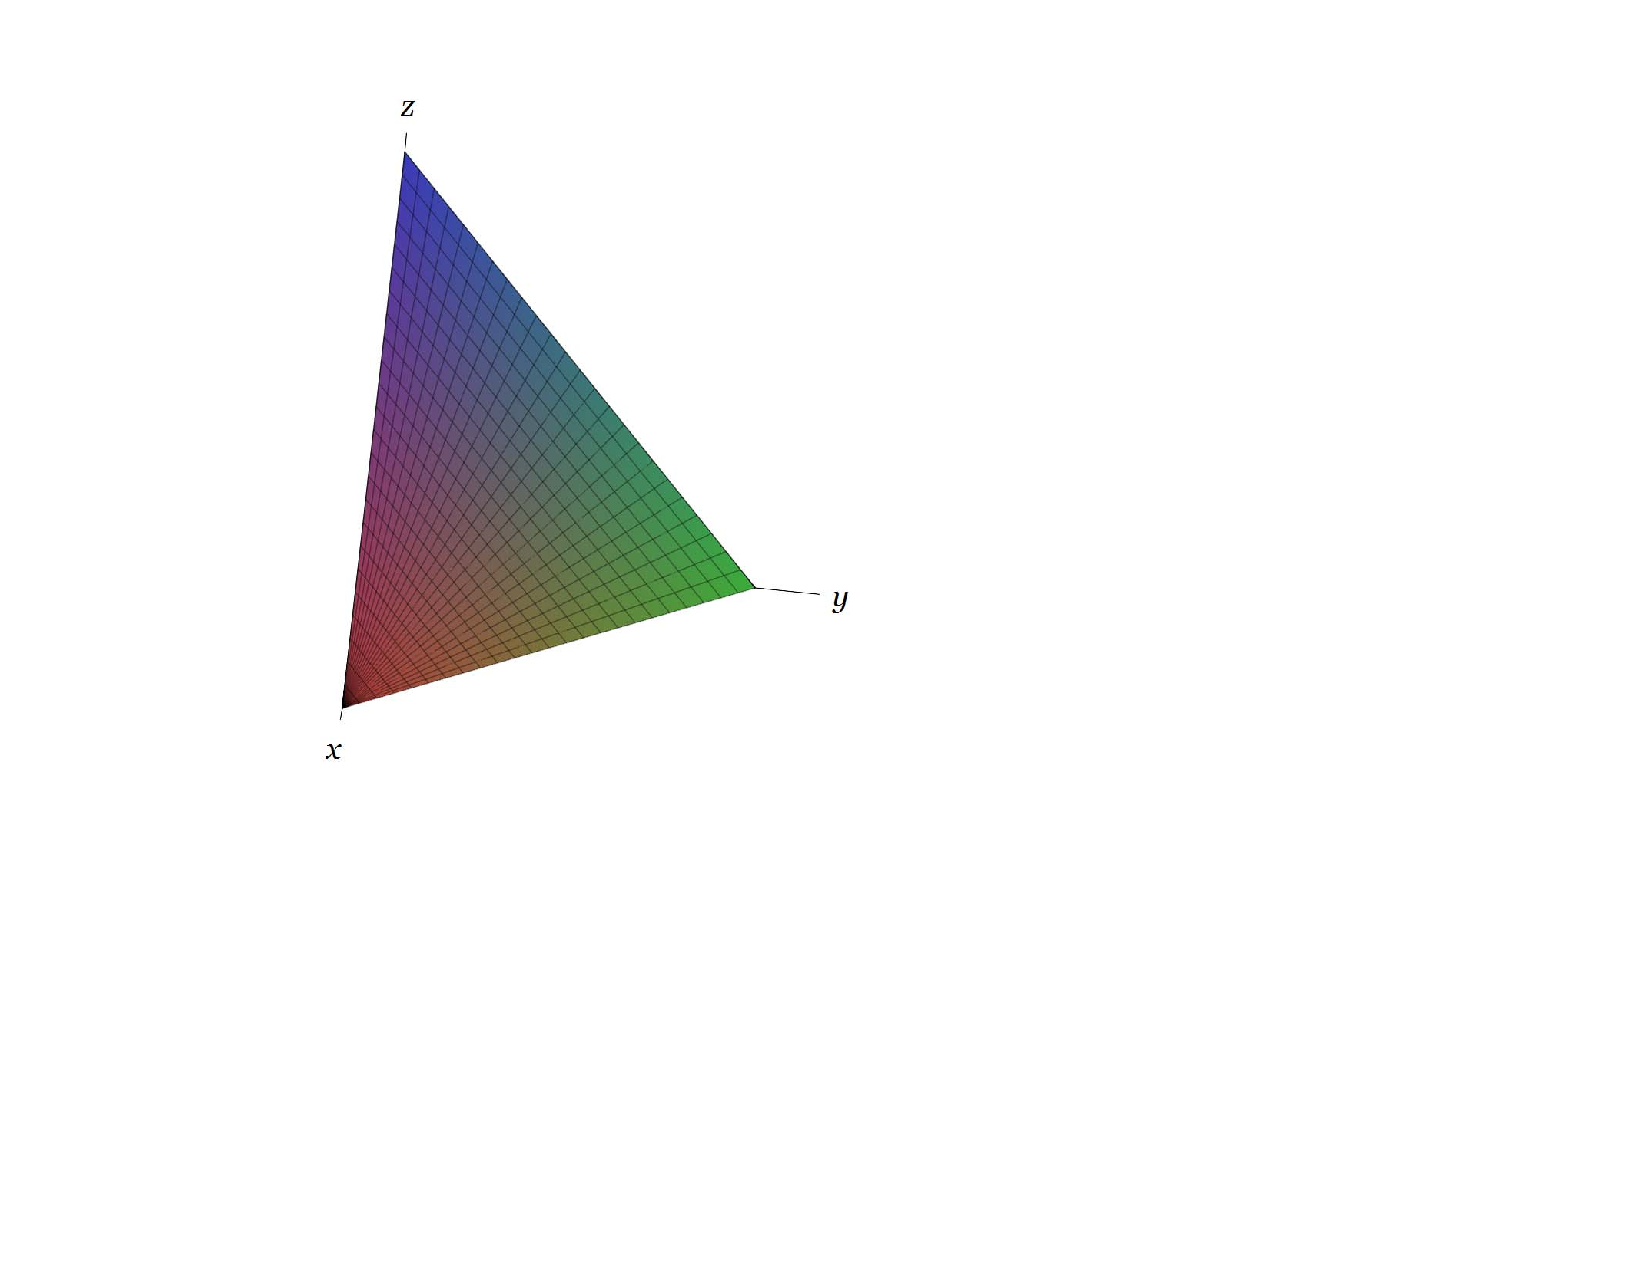
\includegraphics[scale=0.4]{volume2.pdf}
\end{center}
}}} \fi

\item Reverse the order of integration to $\,dy\,dz\,dx$.

\ifans{\fbox{$\int_0^7 \int_0^{21-3x} \int_0^{3-\frac{3}{7}x-\frac{1}{7}z} 1\,dy\,dz\,dx$}} \fi

\end{enumerate}

\item The solid below is enclosed by $x=0$, $x=1$, $y=0$, $z=0$, $z=1$, and $2x+y+2z=6$.

\begin{center}
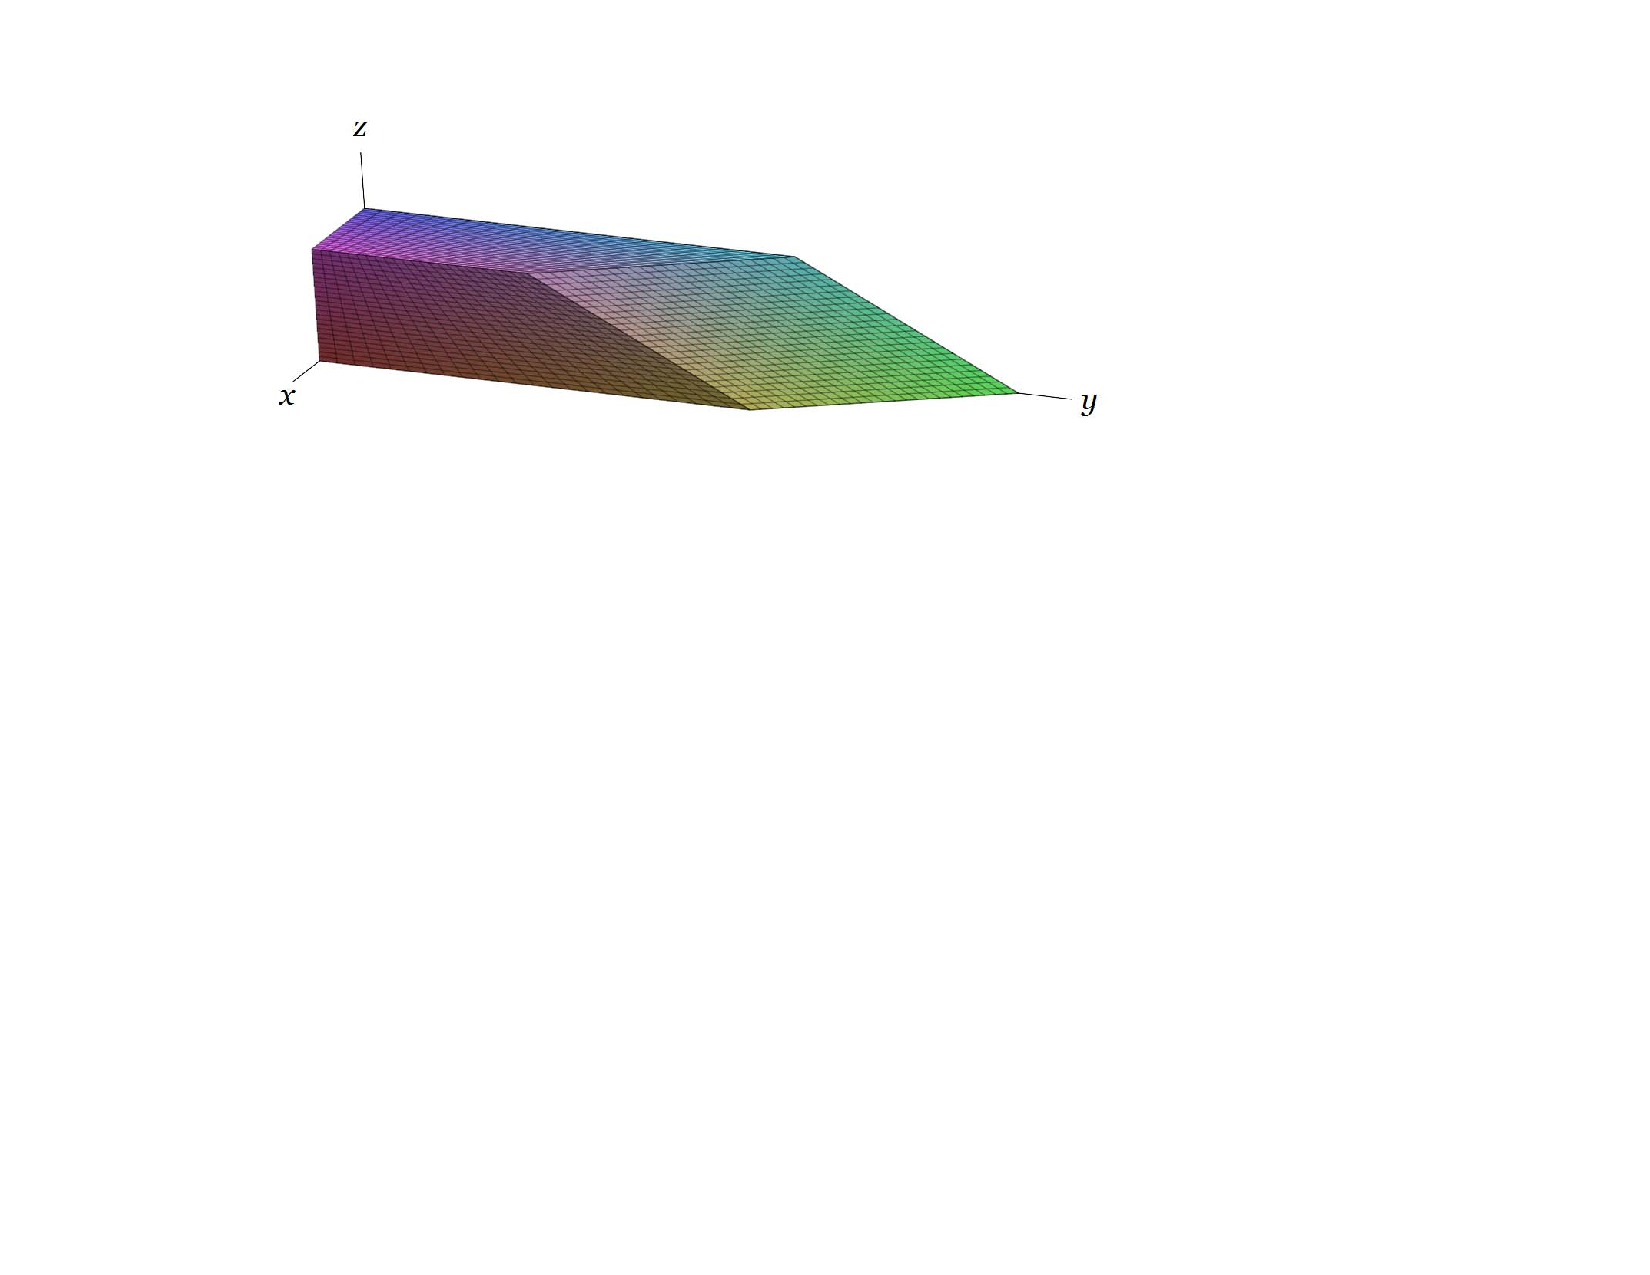
\includegraphics[scale=0.7]{volume.pdf}
\end{center}

\begin{enumerate}

\item Set up a triple integral or triple integrals with the order of integration as \underline{$dydxdz$} which represent(s) the volume of the solid.

\ifans{\fbox{$\int_0^1 \int_0^1 \int_0^{6-2x-2z} 1 \,dy\,dx\,dz$}} \fi

\item Set up a triple integral or triple integrals with the order of integration as \underline{$dzdydx$} which represent(s) the volume of the solid.

\ifans{\fbox{$\int_0^1 \int_0^{4-2x} \int_0^{1} 1 \,dz\,dy\,dx+\int_0^1 \int_{4-2x}^{6-2x} \int_0^{3-x-\frac{1}{2}y} 1 \,dz\,dy\,dx$}} \fi

\end{enumerate}

\item Use a triple integral to calculate the volume of the solid which is bounded by $z=3-x^2$, $z=2x^2$, $y=0$, and $y=1$.

\ifans{\fbox{4}} \fi

\item Use a triple integral to calculate the volume of the solid which is bounded by $z=y+4$, $z=0$, and $x^2+y^2=4$.

\ifans{\fbox{$16\pi$}} \fi

\item The integral $\int_0^{\pi/2} \int_0^{\pi/3} \int_0^1 \rho^2\sin{\phi} \,d\rho\,d\phi\,d\theta$ is given in spherical coordinates.  Sketch a solid whose volume is represented by the value of this integral.

\ifans{\fbox{\parbox{1\linewidth}{The integral can be interpreted as the volume of the solid in the first octant which is contained within the sphere $x^2+y^2+z^2=1$, the cone $z=\frac{1}{\sqrt{3}}\sqrt{x^2+y^2}$, and the planes $x=0$ and $y=0$.
\begin{center}
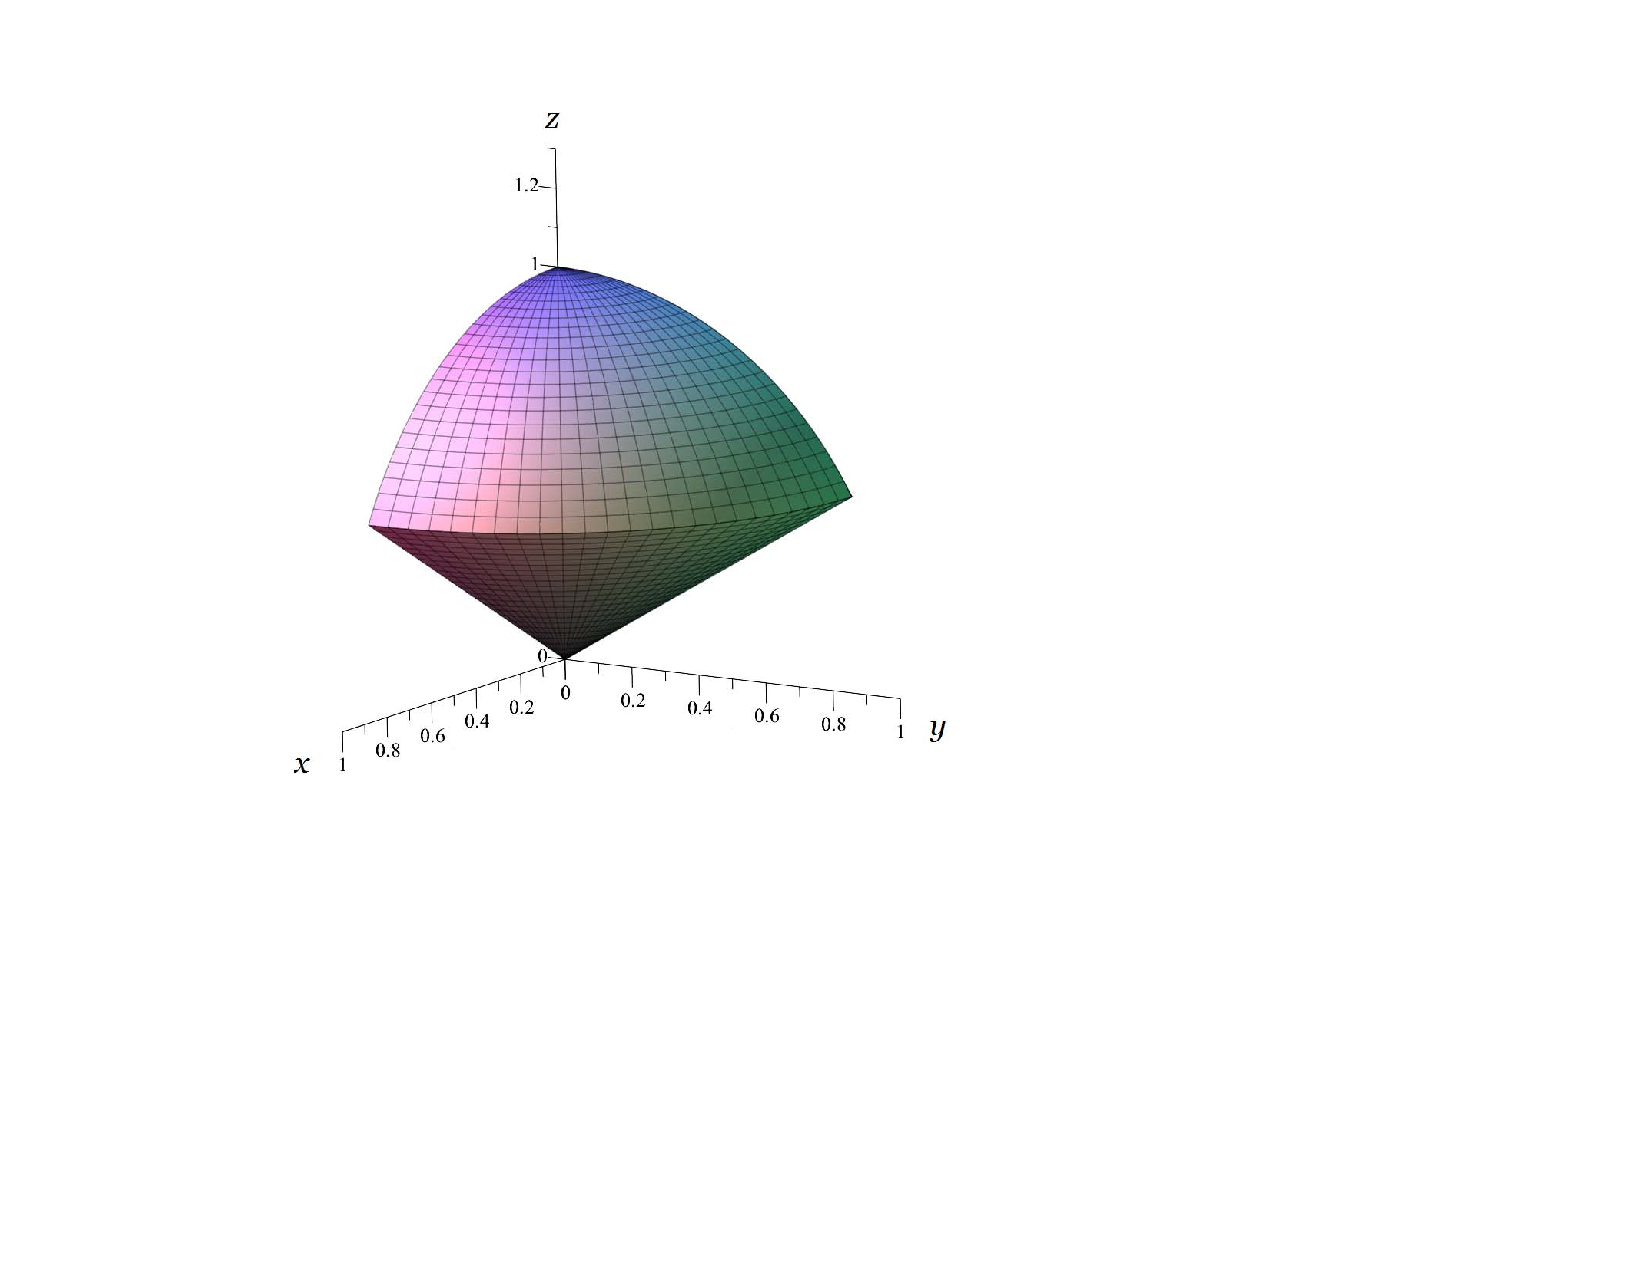
\includegraphics[scale=0.33]{volume3.pdf}
\end{center}
}}} \fi

\item Mario and Luigi run a concession stand in Wario Stadium, ``Missed Jump Creamery," and their top selling product is ice cream cones.  Mario's ice cream cones can be modeled by the solid which is bounded above by $x^2+y^2+z^2=4$ and is bounded below by $z=\sqrt{x^2+y^2}$.  Luigi's ice cream cones can be modeled by the solid which is bounded above by $z=2-x^2-y^2$ and bounded below by $z=\sqrt{x^2+y^2}$. 

\begin{center}
\begin{tabular}{cc}
Mario's Ice Cream Cone & Luigi's Ice Cream Cone\\
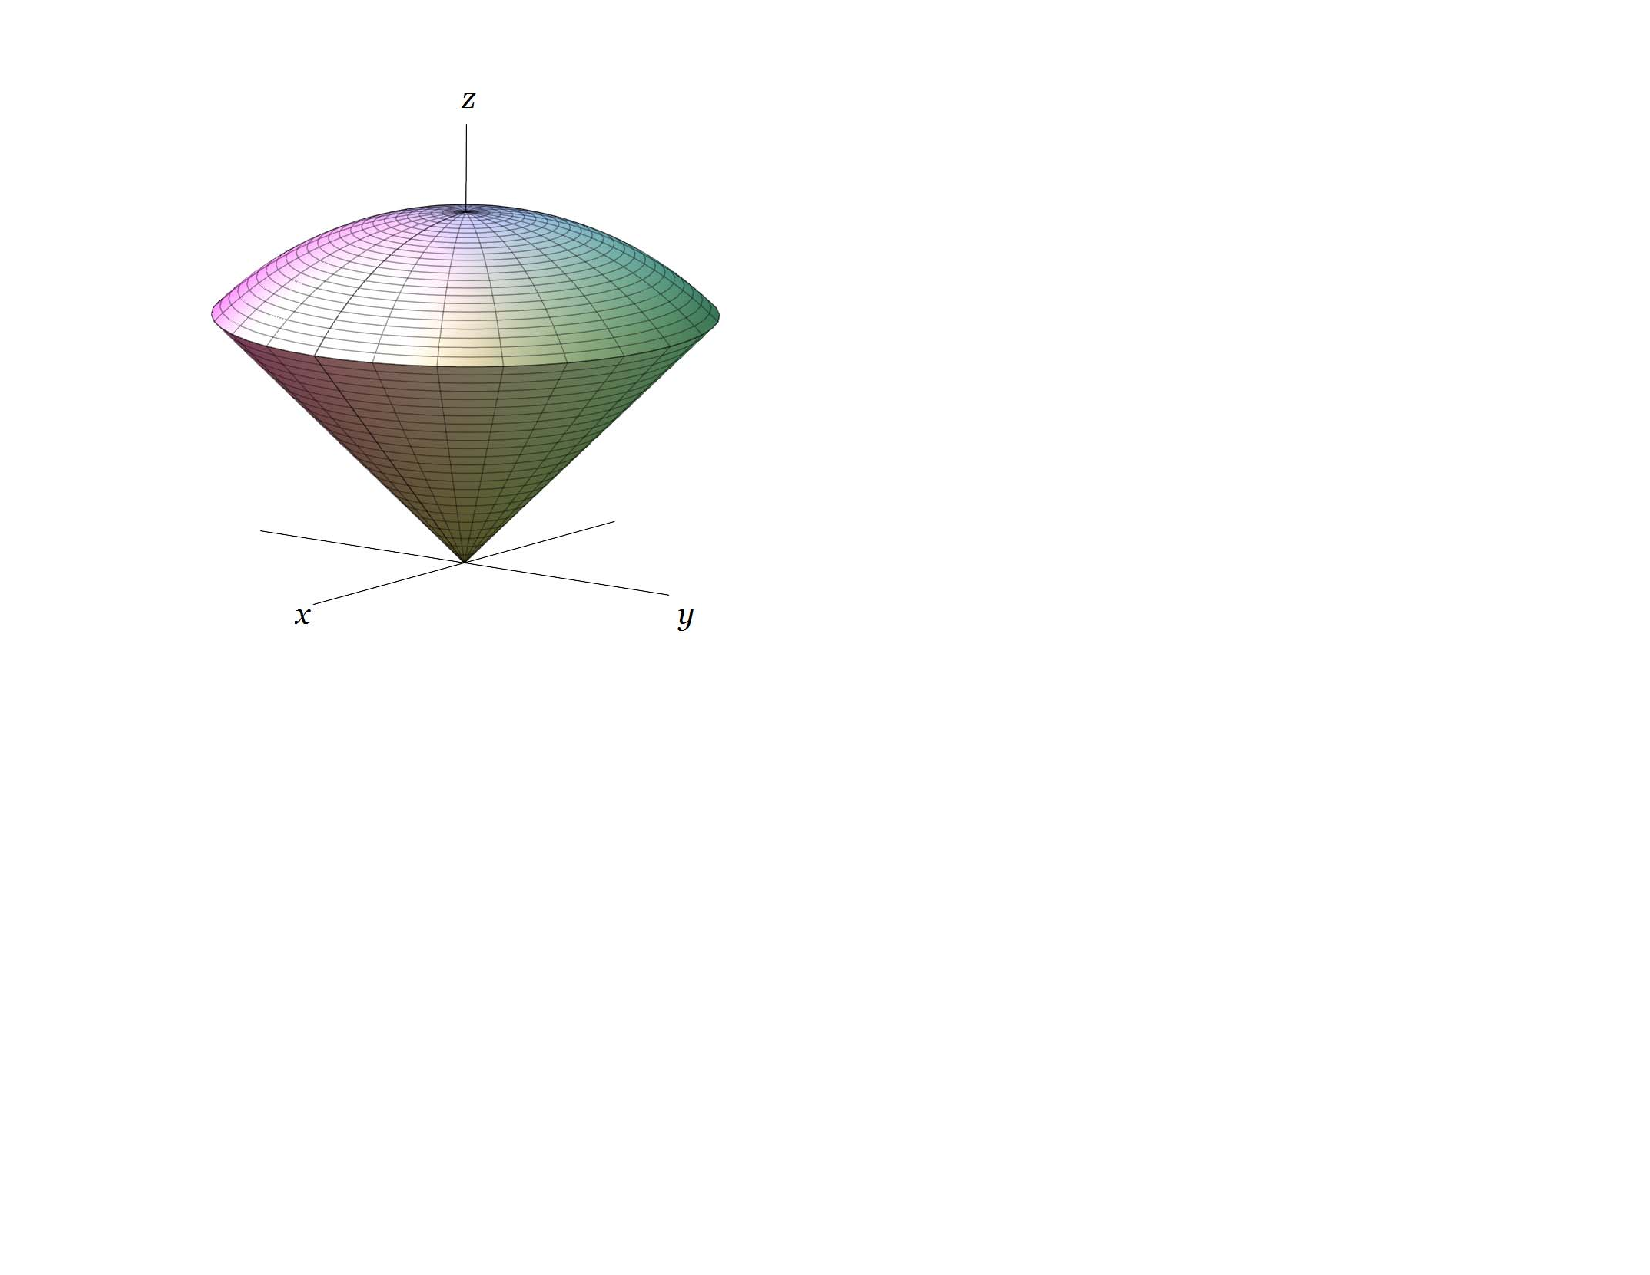
\includegraphics[scale=0.5]{Mario.pdf} & 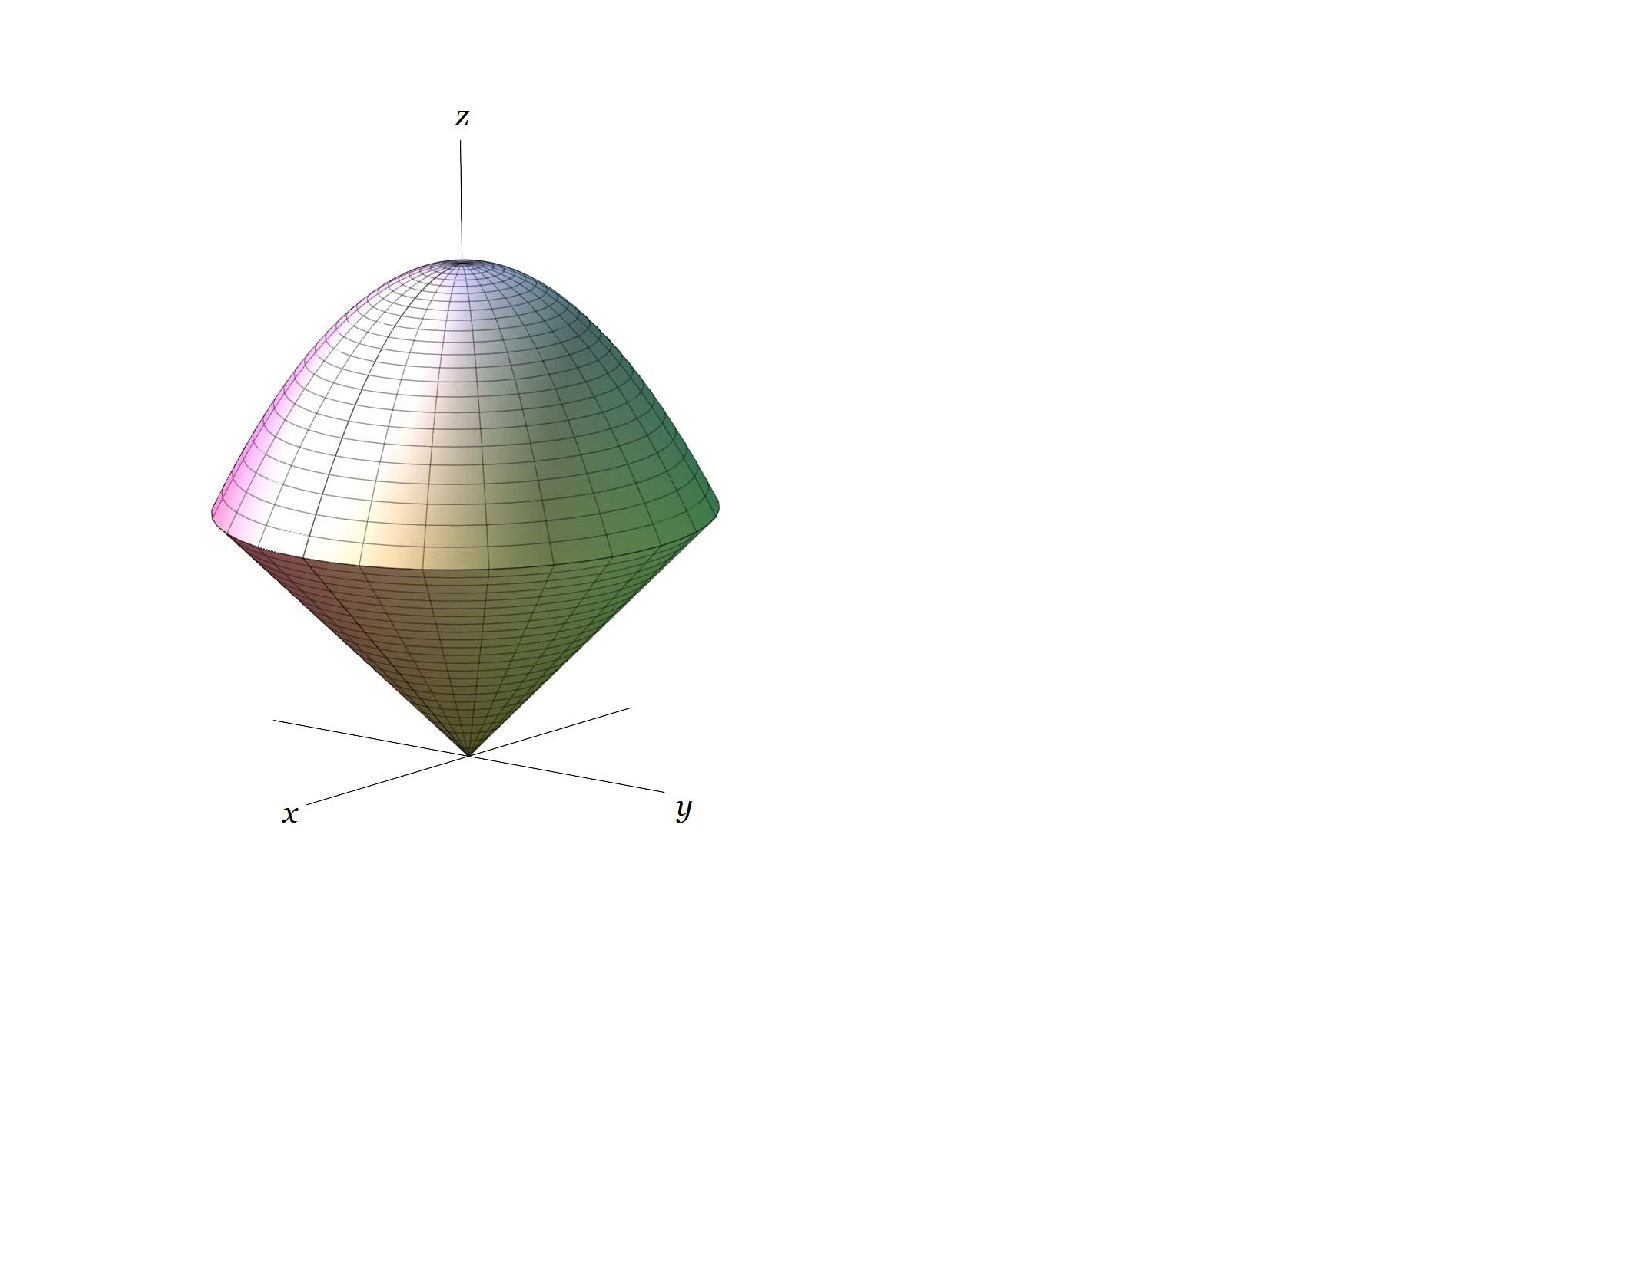
\includegraphics[scale=0.4]{Luigi.pdf}
\end{tabular}\\
(Images are not to scale)
\end{center}

\begin{enumerate}

\item Set up a triple integral in rectangular coordinates which represents the volume of Mario's ice cream cones.

\ifans{\fbox{$V_M=\int_{-\sqrt{2}}^{\sqrt{2}} \int_{-\sqrt{2-x^2}}^{\sqrt{2-x^2}} \int_{\sqrt{x^2+y^2}}^{\sqrt{4-x^2-y^2}} 1 \,dz\,dy\,dx$}} \fi

\item Set up a triple integral in cylindrical coordinates which represents the volume of Mario's ice cream cones.

\ifans{\fbox{$V_M=\int_0^{2\pi} \int_0^{\sqrt{2}} \int_r^{\sqrt{4-r^2}} r\,dz\,dr\,d\theta$}} \fi

\item Set up a triple integral in spherical coordinates which represents the volume of Mario's ice cream cones.

\ifans{\fbox{$V_M=\int_0^{\pi/4} \int_0^{2\pi} \int_0^2 \rho^2 \sin{\phi} \,d\rho \,d\theta \,d\phi$}} \fi

\item Set up a triple integral in rectangular coordinates which represents the volume of Luigi's ice cream cones.

\ifans{\fbox{$V_L=\int_{-1}^{1} \int_{-\sqrt{1-x^2}}^{\sqrt{1-x^2}} \int_{\sqrt{x^2+y^2}}^{2-x^2-y^2} 1 \,dz\,dy\,dx$}} \fi

\item Set up a triple integral in cylindrical coordinates which represents the volume of Luigi's ice cream cones.

\ifans{\fbox{$V_L=\int_0^{2\pi} \int_0^{1} \int_r^{2-r^2} r\,dz\,dr\,d\theta$}} \fi

\item Determine whose ice cream cones have the larger volume.

\ifans{\fbox{\parbox{1\linewidth}{$V_M=\frac{16\pi}{3}\left(1-\frac{\sqrt{2}}{2}\right)\approx 4.907$; $V_L=\frac{5\pi}{6}\approx 2.618$; So, Mario's ice cream cones have the larger volume.}}} \fi

\end{enumerate}

\item Consider the surfaces $x^2+y^2+z^2=16$ and $x^2+y^2=4$, shown below.

\begin{center}
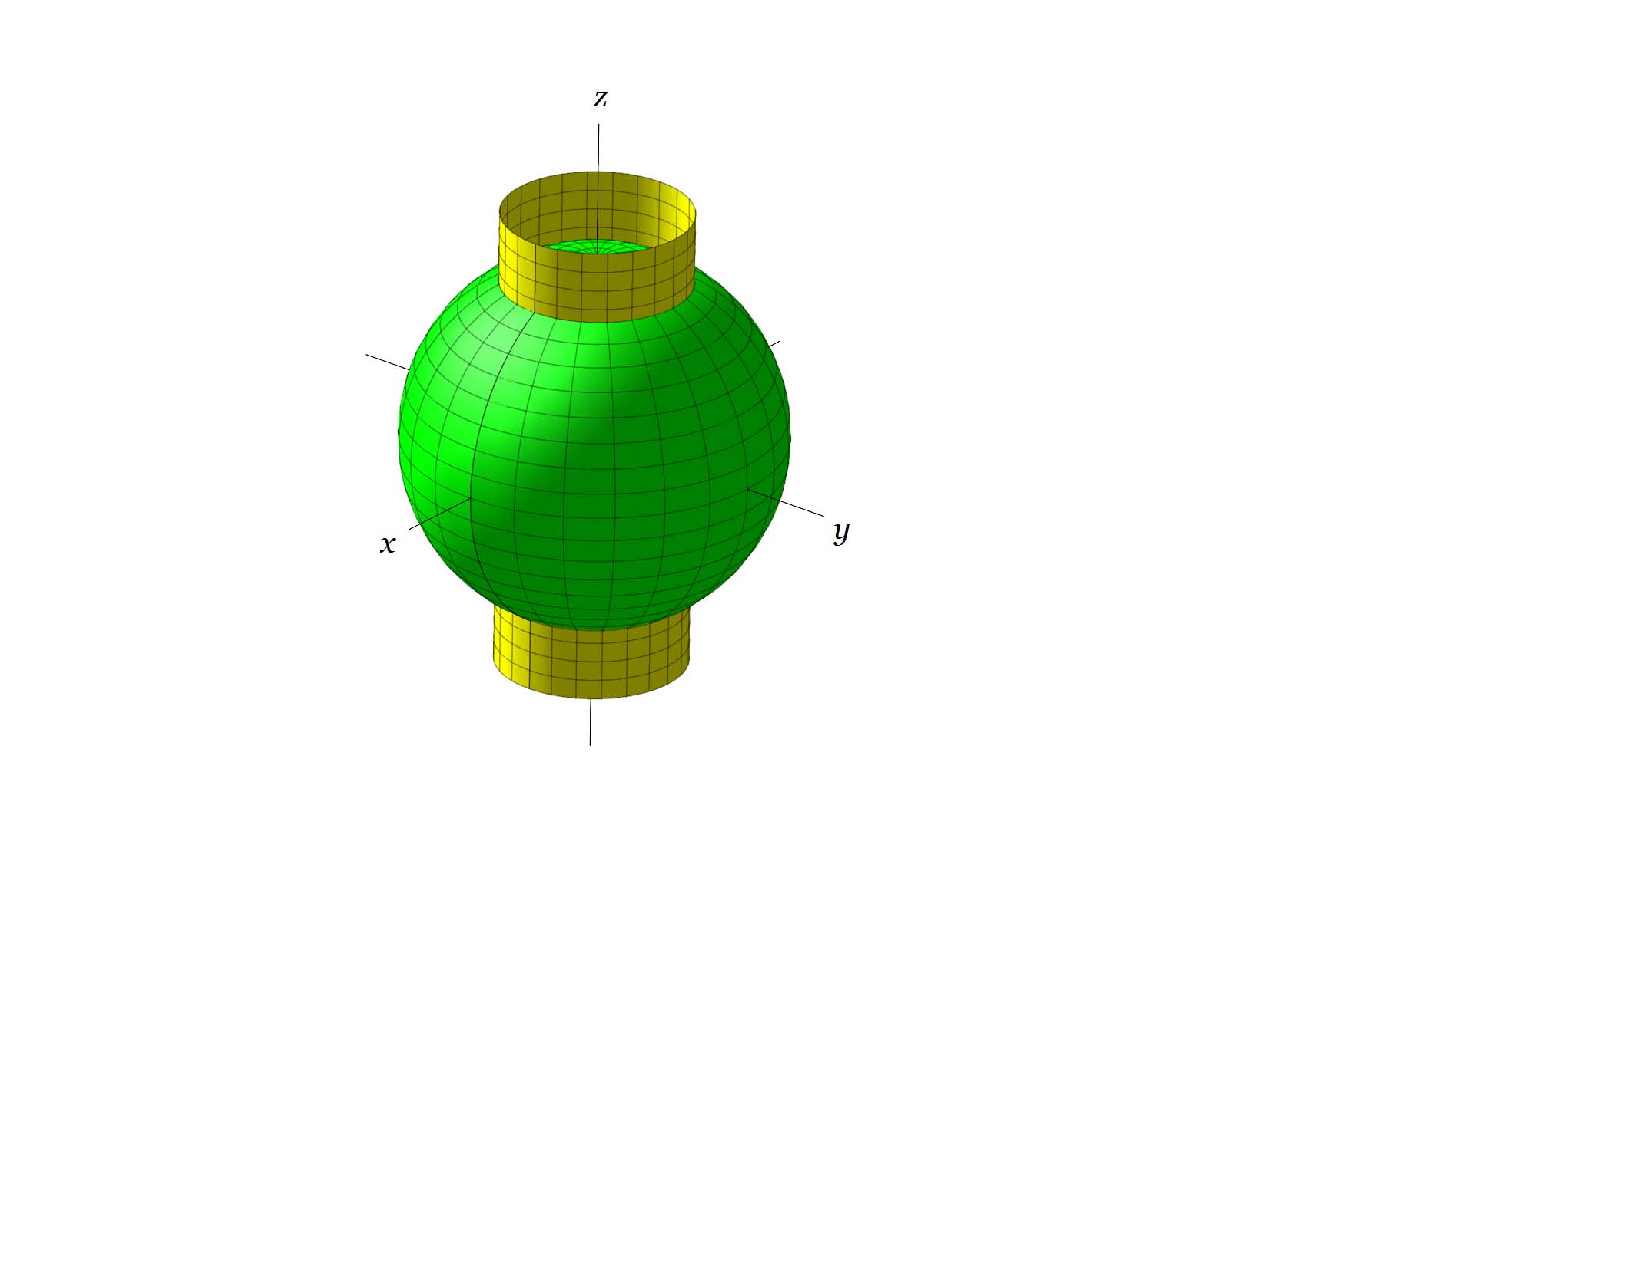
\includegraphics[scale=0.5]{earth.pdf}
\end{center}

\begin{enumerate}

\item Set up a triple integral in cylindrical coordinates which can be used to calculate the volume of the solid which is inside of $x^2+y^2+z^2=16$ but outside of $x^2+y^2=4$.

\ifans{\fbox{$V=\int_0^{2\pi} \int_2^4 \int_{-\sqrt{16-r^2}}^{\sqrt{16-r^2}} r \,dz\,dr\,d\theta$}} \fi

\item Set up a triple integral in spherical coordinates which can be used to calculate the volume of the solid which is inside of $x^2+y^2+z^2=16$ but outside of $x^2+y^2=4$.

\ifans{\fbox{$V=\int_0^{2\pi} \int_{\pi/6}^{5\pi/6} \int_{2\csc{\phi}}^4 \rho^2\sin{\phi} \,d\rho\,d\phi\,d\theta$}} \fi

\item Calculate the volume of the solid which is inside of $x^2+y^2+z^2=16$ but outside of $x^2+y^2=4$ by evaluating one of your integrals from parts (a) or (b).

\ifans{\fbox{$32\pi\sqrt{3}$}} \fi

\end{enumerate}

\item Convert the integral $\int_0^4 \int_{-\sqrt{4-(y-2)^2}}^{\sqrt{4-(y-2)^2}} \int_0^{\sqrt{4-x^2-y^2}} xyz \,dz\,dx\,dy$ from rectangular coordinates to cylindrical coordinates.

\ifans{\fbox{$\int_0^\pi \int_0^{4\sin{\theta}} \int_0^{\sqrt{4-r^2}} r^3z\cos{\theta}\sin{\theta} \,dz\,dr\,d\theta$}} \fi

\item Consider the integral $\int_{-3}^3 \int_0^{\sqrt{9-y^2}} \int_0^{\sqrt{9-x^2-y^2}} (x^2+y^2) \,dz\,dx\,dy$.

\begin{enumerate}

\item Convert the given integral from rectangular coordinates to cylindrical coordinates.

\ifans{\fbox{$\int_{-\pi/2}^{\pi/2} \int_0^3 \int_0^{\sqrt{9-r^2}} r^3 \,dz\,dr\,d\theta$}} \fi

\item Convert the given integral from rectangular coordinates to spherical coordinates.

\ifans{\fbox{$\int_0^{\pi/2} \int_{-\pi/2}^{\pi/2} \int_0^3 \rho^4\sin^3{\phi}\,d\rho\,d\theta\,d\phi$}} \fi

\end{enumerate}

\end{enumerate}

\end{document}